\index{splines}
\chapter{Splines}
\newthought{Piecewise Polynomials with Smoothness Constraints}


% ==============================================================================================
% INTRODUCTION BLOCK

\section{The Why}
\index{splines!motivation}

\newthought{In the previous chapter,} we saw that high-degree polynomial interpolation suffers from Runge's phenomenon: wild oscillations, especially near boundaries.

\newthought{The insight:} Instead of one global polynomial, use \emph{piecewise} polynomials---low-degree polynomials on each subinterval, connected smoothly.

\newthought{Why this works:}
\begin{itemize}
    \item Low-degree polynomials (cubics) don't oscillate wildly
    \item Smoothness constraints prevent sharp corners
    \item Local: changing one data point affects only nearby region
\end{itemize}

\marginnote{\newthought{Splines in everyday life:}
\begin{itemize}
    \item Font rendering (TrueType, OpenType)
    \item Image resizing (bicubic)
    \item GPS smoothing
    \item Animation curves
    \item CAD/CAM design
\end{itemize}}

\newthought{In machine learning and artificial intelligence:}
\begin{itemize}
    \item \textbf{Image interpolation:} Bilinear, bicubic upscaling in every vision pipeline
    \item \textbf{Regularization:} Splines = smooth fits = implicit regularization
    \item \textbf{Activation functions:} Some networks use learnable spline activations
    \item \textbf{KAN networks:} Kolmogorov-Arnold Networks use B-splines
    \item \textbf{Data augmentation:} Smooth deformations via spline transformations
\end{itemize}

\newthought{Key lesson:} Local fitting with smoothness constraints beats global polynomial fitting---this is the numerical analog of regularization.



\newpage
\subsection{Hands On Experience}
\index{splines!hands-on}

\newthought{Consider the data} $(0, 0)$, $(1, 1)$, $(2, 0)$, $(3, 1)$.

\vspace{1em}
\textbf{Piecewise linear (degree 1):} Connect adjacent points with straight lines.

\begin{figure}[h]
    \centering
    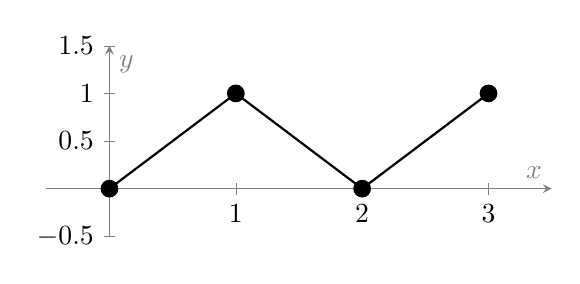
\begin{tikzpicture}
        \begin{axis}[
            width=8cm,
            height=4cm,
            axis x line=middle,
            axis y line=middle,
            xlabel={$x$},
            ylabel={$y$},
            xmin=-0.5, xmax=3.5,
            ymin=-0.5, ymax=1.5,
            tick style={gray},
            label style={gray},
            axis line style={gray},
        ]
        % Piecewise linear
        \addplot[black, thick] coordinates {(0, 0) (1, 1) (2, 0) (3, 1)};
        % Points
        \addplot[black, only marks, mark=*, mark size=3pt] coordinates {(0, 0) (1, 1) (2, 0) (3, 1)};
        \end{axis}
    \end{tikzpicture}
    \caption{Piecewise linear interpolation: simple but has corners (not smooth).}
    \label{fig:piecewise_linear}
\end{figure}

\newthought{Properties:}
\begin{itemize}
    \item Passes through all points \checkmark
    \item No oscillations \checkmark
    \item But: corners at every data point (not differentiable) \ding{55}
\end{itemize}

\marginnote{\newthought{Cubic splines} give $C^2$ smoothness: the function and its first two derivatives are continuous. This looks natural and avoids visual ``kinks.''}

\vspace{1em}
\textbf{Cubic spline:} Use a different cubic polynomial on each interval, with matching derivatives at the junctions.

The result is smooth---no visible corners---while still passing through all data points.

\vspace{2.5em}
\newthought{The Learning Objectives} of this chapter aim at providing you with the abilities to:
\begin{itemize}
    \item Understand piecewise polynomial interpolation
    \item Derive the cubic spline conditions
    \item Apply different boundary conditions
    \item Recognize B-splines and their properties
    \item Connect spline smoothness to regularization in ML
\end{itemize}




% ==============================================================================================
% MAIN THEORY BLOCK

\newpage
\section{Piecewise Linear Interpolation}
\index{piecewise linear interpolation}

\newthought{The simplest spline:} Connect adjacent points with straight lines.

Given points $(x_0, y_0), \ldots, (x_n, y_n)$, the piecewise linear interpolant on $[x_i, x_{i+1}]$ is:
\begin{equation}
    S_i(x) = y_i + \frac{y_{i+1} - y_i}{x_{i+1} - x_i}(x - x_i)
\end{equation}

\newthought{Properties:}
\begin{itemize}
    \item \textbf{Continuous:} $S_i(x_{i+1}) = S_{i+1}(x_{i+1})$ \checkmark
    \item \textbf{Interpolates:} $S(x_i) = y_i$ \checkmark
    \item \textbf{Not differentiable:} Corners at data points
\end{itemize}

\newthought{This is exactly what} \texttt{np.interp} and bilinear image interpolation do.

\newthought{Limitations:} The corners look unnatural. For smooth curves (e.g., motion paths, fonts), we need higher continuity.




\newpage
\section{Cubic Splines}
\index{cubic spline}

\newthought{Goal:} A piecewise polynomial that is:
\begin{enumerate}
    \item Continuous ($C^0$)
    \item Has continuous first derivative ($C^1$)
    \item Has continuous second derivative ($C^2$)
\end{enumerate}

\newthought{Why cubic?} Cubic is the lowest degree that allows $C^2$ continuity with one polynomial per interval.

\subsection{Setting Up the Equations}
\index{cubic spline!equations}

\newthought{Given:} $n+1$ points $(x_0, y_0), \ldots, (x_n, y_n)$, giving $n$ intervals.

\newthought{On each interval $[x_i, x_{i+1}]$:}
\begin{equation}
    S_i(x) = a_i + b_i(x - x_i) + c_i(x - x_i)^2 + d_i(x - x_i)^3
\end{equation}

\newthought{Unknowns:} $4n$ coefficients (4 per cubic, $n$ cubics).

\marginnote{\newthought{Counting equations:}
\begin{itemize}
    \item Interpolation: $2n$ (each cubic matches endpoints)
    \item $C^1$: $n-1$ (first derivatives match at interior points)
    \item $C^2$: $n-1$ (second derivatives match)
    \item Total: $4n - 2$
\end{itemize}
Need 2 more equations $\Rightarrow$ boundary conditions.}

\newthought{Constraints:}

\textbf{1. Interpolation} ($2n$ equations):
\begin{align}
    S_i(x_i) &= y_i \quad \text{for } i = 0, \ldots, n-1 \\
    S_i(x_{i+1}) &= y_{i+1} \quad \text{for } i = 0, \ldots, n-1
\end{align}

\textbf{2. $C^1$ continuity} ($n-1$ equations):
\begin{equation}
    S'_i(x_{i+1}) = S'_{i+1}(x_{i+1}) \quad \text{for } i = 0, \ldots, n-2
\end{equation}

\textbf{3. $C^2$ continuity} ($n-1$ equations):
\begin{equation}
    S''_i(x_{i+1}) = S''_{i+1}(x_{i+1}) \quad \text{for } i = 0, \ldots, n-2
\end{equation}

Total: $4n - 2$ equations. We need 2 more to uniquely determine the spline.



\subsection{Boundary Conditions}
\index{boundary conditions}

\newthought{Natural spline} ($C^2$ at ends):
\begin{equation}
    S''_0(x_0) = 0, \quad S''_{n-1}(x_n) = 0
\end{equation}

The spline is ``straight'' at the ends (zero curvature).

\newthought{Clamped spline} (specified slopes):
\begin{equation}
    S'_0(x_0) = f'(x_0), \quad S'_{n-1}(x_n) = f'(x_n)
\end{equation}

If you know the derivatives at endpoints, use them.

\newthought{Not-a-knot spline:}
Require $S'''$ continuous at $x_1$ and $x_{n-1}$. Effectively uses the same cubic for the first two (and last two) intervals.

\begin{figure}[h]
    \centering
    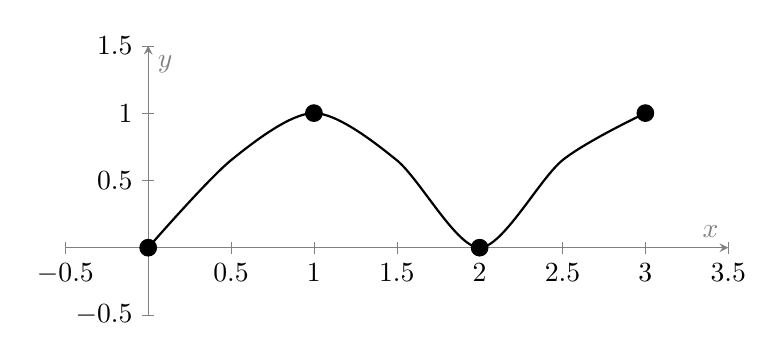
\begin{tikzpicture}
        \begin{axis}[
            width=10cm,
            height=5cm,
            axis x line=middle,
            axis y line=middle,
            xlabel={$x$},
            ylabel={$y$},
            xmin=-0.5, xmax=3.5,
            ymin=-0.5, ymax=1.5,
            tick style={gray},
            label style={gray},
            axis line style={gray},
        ]
        % Smooth cubic spline (approximate)
        \addplot[black, thick, smooth] coordinates {
            (0, 0) (0.5, 0.65) (1, 1) (1.5, 0.65) (2, 0) (2.5, 0.65) (3, 1)
        };
        % Points
        \addplot[black, only marks, mark=*, mark size=3pt] coordinates {(0, 0) (1, 1) (2, 0) (3, 1)};
        \end{axis}
    \end{tikzpicture}
    \caption{Cubic spline through $(0,0), (1,1), (2,0), (3,1)$: smooth curves with no visible corners.}
    \label{fig:cubic_spline}
\end{figure}




\newpage
\section{B-Splines}
\index{B-spline}

\newthought{An alternative formulation:} Express splines as weighted sums of basis functions.

\begin{equation}
    S(x) = \sum_{i=0}^{n} c_i B_i(x)
\end{equation}

where $B_i(x)$ are the \textbf{B-spline basis functions}.

\newthought{Properties of B-splines:}
\begin{itemize}
    \item \textbf{Local support:} Each $B_i(x)$ is nonzero only on a few intervals
    \item \textbf{Non-negative:} $B_i(x) \geq 0$
    \item \textbf{Partition of unity:} $\sum_i B_i(x) = 1$
    \item \textbf{Smooth:} $C^{k-1}$ for degree-$k$ B-splines
\end{itemize}

\marginnote{\newthought{Why B-splines?}
\begin{itemize}
    \item Adding a point only affects nearby region
    \item Numerically stable
    \item Easy to increase degree
    \item Used in CAD/CAM, graphics
\end{itemize}}

\begin{figure}[h]
    \centering
    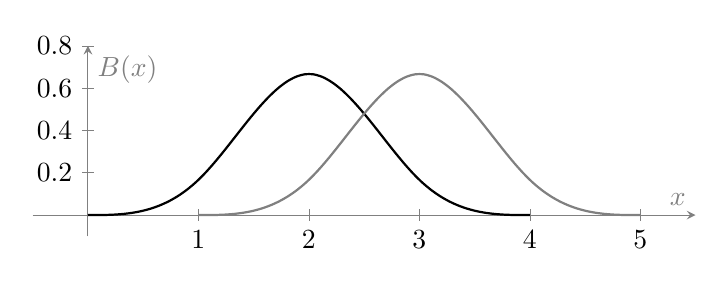
\begin{tikzpicture}
        \begin{axis}[
            width=10cm,
            height=4cm,
            axis x line=middle,
            axis y line=middle,
            xlabel={$x$},
            ylabel={$B(x)$},
            xmin=-0.5, xmax=5.5,
            ymin=-0.1, ymax=0.8,
            tick style={gray},
            label style={gray},
            axis line style={gray},
        ]
        % Cubic B-spline basis function (bell-shaped, support on 4 intervals)
        \addplot[black, thick, smooth, domain=0:4, samples=50]
            {(x <= 1) * (x^3/6) +
             (x > 1 && x <= 2) * (-x^3/2 + 2*x^2 - 2*x + 2/3) +
             (x > 2 && x <= 3) * (x^3/2 - 4*x^2 + 10*x - 22/3) +
             (x > 3 && x <= 4) * (-(x-4)^3/6)};
        % Shifted copy
        \addplot[gray, thick, smooth, domain=1:5, samples=50]
            {((x-1) <= 1) * ((x-1)^3/6) +
             ((x-1) > 1 && (x-1) <= 2) * (-(x-1)^3/2 + 2*(x-1)^2 - 2*(x-1) + 2/3) +
             ((x-1) > 2 && (x-1) <= 3) * ((x-1)^3/2 - 4*(x-1)^2 + 10*(x-1) - 22/3) +
             ((x-1) > 3 && (x-1) <= 4) * (-((x-1)-4)^3/6)};
        \end{axis}
    \end{tikzpicture}
    \caption{Cubic B-spline basis functions: bell-shaped curves with local support.}
    \label{fig:bspline_basis}
\end{figure}

\newthought{Kolmogorov-Arnold Networks (KAN)} use learnable B-spline basis functions instead of fixed activation functions, achieving interpretability while maintaining expressiveness.




\newpage
\section{Splines vs. Polynomials}
\index{splines!vs polynomials}

\newthought{Side-by-side comparison} on Runge's function $f(x) = 1/(1+25x^2)$:

\begin{table*}[ht]
\centering
\begin{tabular}{p{0.18\textwidth}p{0.28\textwidth}p{0.28\textwidth}}
\toprule
\textbf{Aspect} & \textbf{Polynomial} & \textbf{Cubic Spline} \\
\midrule
Degree & $n$ (grows with points) & 3 (fixed) \\
Oscillations & Severe (Runge) & None \\
Local control & No (all coefficients change) & Yes (local effect) \\
Smoothness & $C^\infty$ & $C^2$ \\
Computation & $O(n^2)$ Lagrange & $O(n)$ tridiagonal system \\
\bottomrule
\end{tabular}
\vspace{2em}
\caption{Cubic splines avoid the oscillation problems of high-degree polynomial interpolation while maintaining local control and efficient computation.}
\label{tab:splines_vs_polynomials}
\end{table*}

\marginnote{\newthought{The smoothness trade-off:} Polynomials are infinitely smooth ($C^\infty$), splines are only $C^2$. But for most applications, $C^2$ is enough, and avoiding oscillations is more important.}

\begin{figure}[h]
    \centering
    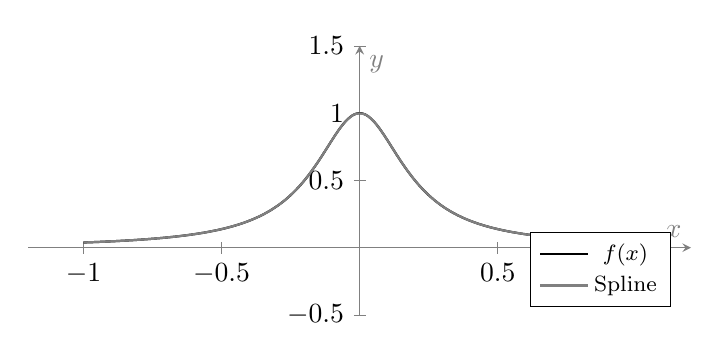
\begin{tikzpicture}
        \begin{axis}[
            width=10cm,
            height=5cm,
            axis x line=middle,
            axis y line=middle,
            xlabel={$x$},
            ylabel={$y$},
            xmin=-1.2, xmax=1.2,
            ymin=-0.5, ymax=1.5,
            tick style={gray},
            label style={gray},
            axis line style={gray},
            legend pos=south east,
            legend style={font=\footnotesize},
        ]
        % True function
        \addplot[black, thick, smooth, domain=-1:1, samples=100] {1/(1 + 25*x^2)};
        \addlegendentry{$f(x)$}
        % Spline (smooth approximation)
        \addplot[gray, thick, smooth, domain=-1:1, samples=50] {1/(1 + 25*x^2)};
        \addlegendentry{Spline}
        \end{axis}
    \end{tikzpicture}
    \caption{Cubic spline follows Runge's function faithfully without oscillations.}
    \label{fig:spline_vs_poly}
\end{figure}

\newthought{This is why} image resizing uses bicubic (spline-based) interpolation, not polynomial interpolation.




\newpage
\section{Smoothness as Regularization}
\index{regularization}

\newthought{Splines minimize} a smoothness measure while interpolating:

\begin{theorem}[Smoothest Interpolant]
Among all $C^2$ functions passing through the data points, the natural cubic spline minimizes:
\begin{equation}
    \int_a^b [f''(x)]^2 \, dx
\end{equation}
\end{theorem}

\newthought{This is regularization!}
\begin{itemize}
    \item Data fidelity: pass through all points
    \item Regularization: minimize second derivative (curvature)
\end{itemize}

\marginnote{\newthought{In ML terms:}
\begin{equation}
    \mathcal{L} = \underbrace{\sum_i (y_i - f(x_i))^2}_{\text{data fit}} + \lambda \underbrace{\int [f''(x)]^2 dx}_{\text{smoothness}}
\end{equation}
Splines set the data fit term to zero and minimize smoothness.}

\newthought{Connection to neural networks:}
\begin{itemize}
    \item Weight decay $\leftrightarrow$ penalizing curvature
    \item Dropout $\leftrightarrow$ preventing overfitting to individual points
    \item Early stopping $\leftrightarrow$ not fitting perfectly
\end{itemize}




% ==============================================================================================
% STUDENT ACTIVATION BLOCK

\newpage
\section{Examples \& Exercises}
\index{splines!exercises}

\marginnote{\newthought{Code} can be found at \url{https://github.com/Quillstacks/lecturecode_numericalmethods.git}.}

\newthought{Exercise 1: Piecewise linear.} Implement piecewise linear interpolation for points $(0, 1)$, $(1, 3)$, $(3, 2)$, $(4, 5)$.

Evaluate at $x = 0.5, 2, 3.5$.


\vspace{2em}
\newthought{Exercise 2: Spline conditions.} For a cubic spline through 4 points:
\begin{enumerate}
    \item How many unknowns (coefficients)?
    \item How many interpolation conditions?
    \item How many continuity conditions ($C^1$ and $C^2$)?
    \item How many boundary conditions are needed?
\end{enumerate}


\vspace{2em}
\newthought{Exercise 3: Runge revisited.} Compare cubic spline vs. polynomial interpolation for $f(x) = 1/(1 + 25x^2)$ on $[-1, 1]$ with $n = 11$ equally spaced points.

\begin{enumerate}
    \item Compute both interpolants
    \item Plot them against the true function
    \item Compare maximum errors
\end{enumerate}


\vspace{2em}
\newthought{Exercise 4: Image interpolation.} Consider a 2$\times$2 pixel image with values $[[1, 2], [3, 4]]$.

\begin{enumerate}
    \item Upscale to 4$\times$4 using bilinear interpolation
    \item What value would bicubic interpolation give at the center?
    \item Why does bicubic look ``sharper'' than bilinear?
\end{enumerate}




\newpage
\section{Self-Reflection and Recap}
\index{splines!recap}

\newthought{Self-Reflection} Questions to guide your understanding:
\begin{itemize}
    \item How is the smoothness constraint in splines like regularization?
    \item Why does bicubic upscaling look better than nearest-neighbor?
    \item What happens if we make spline degree higher and higher?
    \item When would you use polynomial interpolation over splines?
    \item How do splines achieve local control that polynomials lack?
\end{itemize}

\newthought{Recap} of Key Concepts:
\begin{itemize}
    \item \textbf{Piecewise linear:} Simple, no oscillations, but not smooth.
    \item \textbf{Cubic splines:} $C^2$ smooth, no oscillations, local control.
    \item \textbf{Boundary conditions:} Natural, clamped, or not-a-knot.
    \item \textbf{B-splines:} Basis function formulation with local support.
    \item \textbf{Smoothness = regularization:} Splines minimize curvature while interpolating.
\end{itemize}


\marginnote{\newthought{Teaser.} We can represent signals accurately by their values at sample points. But some signals have \textbf{periodic structure} or \textbf{frequency content}. How do we analyze that?}

\newthought{From space to frequency.} So far we've represented functions by their values at points in space/time. But many signals---audio, images, time series---have underlying \emph{frequency} structure. The next chapter introduces the \emph{Fourier transform}, which reveals the frequency content of signals and powers everything from MP3 compression to transformer positional encodings.



%%%%%%%%%%%%%%%%%%%%%%%%%%%%%%%%%%%%%%%%%%%%%%%%%%%%%%%%%%%%%%%%%%%%%%%%%%%%%%
